\documentclass{standalone}
\usepackage{tikz}

\usepackage{braket} % quantum notation
\usepackage{qcircuit} % quantum circuits
\usepackage{pgfplots}

\usetikzlibrary{tikzmark,positioning,automata}
\usetikzlibrary{shapes.geometric}

\pgfplotsset{every axis/.append style={
	label style = {font=\scriptsize},
	tick label style = {font=\scriptsize}
}}

\begin{document}
	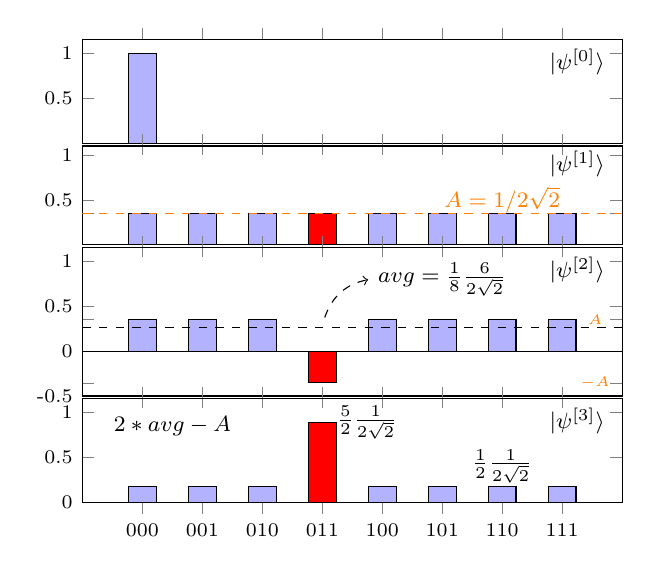
\begin{tikzpicture}
		\begin{axis}[
		%axis equal image, 
		%axis equal top,
		unit vector ratio* = 1 1.5 1,
		%scale only axis = true,
		ymin=0, ymax= 1.15, ybar,
		xmin=0, xmax= 9,
		xtick={1,2,3,4,5,6,7,8}, 
		xticklabels = {},
		ytick = {0.5, 1},
		yticklabels = {0.5,1},
		%symbolic x coords = {a1,a2,a3,a4,a5,a6,a7,a8} ,
		name= firstplot]
			\addplot[draw=black, fill=blue!30] coordinates {
				(1,1)
				(2,0)
				(3,0)
				(4,0)
				(5,0)
				(6,0)
				(7,0)
				(8,0)
			};
		\node[]() at (axis cs:8.25,0.9){{\footnotesize $\ket{\psi^{[0]}}$}};
		\end{axis}
		\begin{axis}[
		unit vector ratio* = 1 1.5 1,
		ymin=0, ymax= 1.1, ybar, 
		xmin=0, xmax= 9, 
		xtick={1,2,3,4,5,6,7,8}, 
		xticklabels = {},
		ytick = {-0.5,0.3535,0.5, 1},
		yticklabels = {-0.5,,0.5,1},
		bar shift = 0pt,
		%symbolic x coords = {a1,a2,a3,a4,a5,a6,a7,a8} ,
		name= secondplot, at=(firstplot.south), anchor = north, yshift=-1pt]
			\addplot[draw=black, fill=blue!30]  coordinates {
				(1,0.3535) 
				(2,0.3535)
				(3,0.3535)
				(4,0.3535)
				(5,0.3535)
				(6,0.3535)
				(7,0.3535)
				(8,0.3535)};
			\addplot[fill=red] coordinates {(4,0.3535)};
			%\node[orange] at (axis cs:7.15,0.42){\tiny $A=1/2\sqrt{2}$};
			\addplot[orange, sharp plot, dashed, update limits = false]
			coordinates {(0,0.3535)(9,0.3535)}
			node[](pt1) at (axis cs:7,0.5){\footnotesize  $A=1/2\sqrt{2}$};
			\node[]() at (axis cs:8.25,0.9){{\footnotesize $\ket{\psi^{[1]}}$}};
		\end{axis}
		\begin{axis}[
		unit vector ratio* = 1 1.5 1,
		ymin=-0.5, ymax= 1.15, ybar, 
		ytick={0}, 
		xmin=0, xmax= 9, 
		xtick={1,2,3,4,5,6,7,8}, 
		xticklabels = {},
		ytick = {-0.5,-0.3535,0,0.3535,0.5, 1},
		yticklabels = {-0.5,,0, ,0.5,1},
		bar shift = 0pt,
		%symbolic x coords = {a1,a2,a3,a4,a5,a6,a7,a8} ,
		name= thirdplot, at=(secondplot.south), anchor = north, yshift=-1pt]
		\addplot[draw=black, fill=blue!30]  coordinates {
			(1,0.3535) 
			(2,0.3535)
			(3,0.3535)
			%(4,0.3535)
			(5,0.3535)
			(6,0.3535)
			(7,0.3535)
			(8,0.3535)};
		\addplot[fill=red] coordinates {(4,-0.3535)};
		\addplot[black, sharp plot, dashed, update limits = false]
			coordinates {(0,0.2651)(9,0.2651)}
			node[above](pt1) at (axis cs:6,0.5){\footnotesize  ${avg}=\frac{1}{8}\frac{6}{2\sqrt{2}}$};
		\addplot[black, sharp plot, update limits = false]
		coordinates {(0,0)(9,0)};
		\node[orange] at (axis cs:8.55,0.3535){\tiny $A$};
		\node[orange] at (axis cs:8.55,-0.3535){\tiny $-A$};
		
		\node[](pt2) at (axis cs:4,0.2651){};
		\draw[->, dashed] (pt2) to[bend left] (pt1.west);
		\node[]() at (axis cs:8.25,0.9){{\footnotesize $\ket{\psi^{[2]}}$}};
		\end{axis}
		\begin{axis}[
		unit vector ratio* = 1 1.5 1,
		ymin=-0.0, ymax= 1.15, ybar, 
		ytick={0}, 
		xmin=0, xmax= 9, 
		xtick={1,2,3,4,5,6,7,8}, 
		xticklabels = {000,001,010,011,100,101,110,111},
		ytick = {0,0.5, 1},
		yticklabels = {0,0.5,1},
		bar shift = 0pt,
		%symbolic x coords = {a1,a2,a3,a4,a5,a6,a7,a8} ,
		name= thirdplot, at=(thirdplot.south), anchor = north, yshift=-1pt]
		\addplot[draw=black, fill=blue!30]  coordinates {
			(1,0.1767) 
			(2,0.1767)
			(3,0.1767)
			%(4,0.3535)
			(5,0.1767)
			(6,0.1767)
			(7,0.1767)
			(8,0.1767)};
		\addplot[fill=red] coordinates {(4,0.8838)};
		
		
		\node[](pt2) at (axis cs:1.5,0.85){{\footnotesize $2*avg-A$}};
		\node[]() at (axis cs:4.75,0.8838){{\footnotesize $\frac{5}{2}\frac{1}{2\sqrt{2}}$}};
		\node[]() at (axis cs:7,0.4){{\footnotesize $\frac{1}{2}\frac{1}{2\sqrt{2}}$}};
		\node[]() at (axis cs:8.25,0.9){{\footnotesize $\ket{\psi^{[3]}}$}};
		\end{axis}
	\end{tikzpicture}
\end{document}